% !TeX spellcheck = en_US
% !TeX root = DynELA.tex
%
% LaTeX source file of DynELA FEM Code
%
% (c) by Olivier Pantalé 2020
%
\chapter{DynELA Finite Element Method library}

\startcontents[chapters]
\printmyminitoc[2]\LETTRINE{T}he \DynELA~is an Explicit FEM code written in \Cpp~using a Python's interface for creating the Finite Element Models. 

\section{The ColorMap class}

%@DOC:ColorMap::ColorMap
% Automatic documentation generated from the DynELA source code
% Do not change anything in this LaTeX file between the @DOC and the @END keywords.
\textcolor{purple}{\textbf{ColorMap::ColorMap}}\label{ColorMap::ColorMap}\index[DL]{ColorMap!ColorMap}\\
ColorMap class.

This class is used to store information for color maps.
%@END

%@DOC:ColorMap::setColorMap()
% Automatic documentation generated from the DynELA source code
% Do not change anything in this LaTeX file between the @DOC and the @END keywords.
\textcolor{purple}{\textbf{ColorMap::setColorMap(~)}}\label{ColorMap::setColorMap()}\index[DL]{ColorMap!setColorMap(~)}\\
Select the color map.

Select the color map for drawings.
The color map is the one represented here after, from blue for low values (left side of the proposed bar) to red for high values (right side of the proposed bar).
\begin{center}
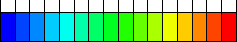
\includegraphics{Figures/ProgrammingLanguage/ColorMap}
\end{center}
%@END

%@DOC:ColorMap::setReverseColorMap()
% Automatic documentation generated from the DynELA source code
% Do not change anything in this LaTeX file between the @DOC and the @END keywords.
\textcolor{purple}{\textbf{ColorMap::setReverseColorMap(~)}}\label{ColorMap::setReverseColorMap()}\index[DL]{ColorMap!setReverseColorMap(~)}\\
Select the color map.

Select the color map for drawings.
The color map is the one represented here after, from red for low values (left side of the proposed bar) to blue for high values (right side of the proposed bar).
\begin{center}
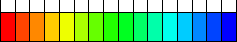
\includegraphics{Figures/ProgrammingLanguage/ReverseColorMap}
\end{center}
%@END

%@DOC:ColorMap::setDeepColorMap()
% Automatic documentation generated from the DynELA source code
% Do not change anything in this LaTeX file between the @DOC and the @END keywords.
\textcolor{purple}{\textbf{ColorMap::setDeepColorMap(~)}}\label{ColorMap::setDeepColorMap()}\index[DL]{ColorMap!setDeepColorMap(~)}\\
Select the deep color map.

Select the deep color map for drawings.
The deep color map is the one represented here after, from dark blue for low values (left side of the proposed bar) to dark red for high values (right side of the proposed bar).
\begin{center}
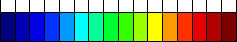
\includegraphics{Figures/ProgrammingLanguage/DeepColorMap}
\end{center}
%@END

%@DOC:ColorMap::setReverseDeepColorMap()
% Automatic documentation generated from the DynELA source code
% Do not change anything in this LaTeX file between the @DOC and the @END keywords.
\textcolor{purple}{\textbf{ColorMap::setReverseDeepColorMap(~)}}\label{ColorMap::setReverseDeepColorMap()}\index[DL]{ColorMap!setReverseDeepColorMap(~)}\\
Select the reversed deep color map.

Select the reversed deep color map for drawings.
The reversed deep color map is the one represented here after, from dark red for low values (left side of the proposed bar) to dark blue for high values (right side of the proposed bar).
\begin{center}
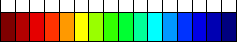
\includegraphics{Figures/ProgrammingLanguage/ReverseDeepColorMap}
\end{center}
%@END

%@DOC:ColorMap::setGrayMap()
% Automatic documentation generated from the DynELA source code
% Do not change anything in this LaTeX file between the @DOC and the @END keywords.
\textcolor{purple}{\textbf{ColorMap::setGrayMap(~)}}\label{ColorMap::setGrayMap()}\index[DL]{ColorMap!setGrayMap(~)}\\
Select the gray color map.

Select the gray color map for drawings.
The gray color map is the one represented here after, from black for low values (left side of the proposed bar) to white for high values (right side of the proposed bar).
\begin{center}
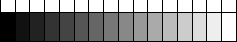
\includegraphics{Figures/ProgrammingLanguage/GrayMap}
\end{center}
%@END

%@DOC:ColorMap::setReverseGrayMap()
% Automatic documentation generated from the DynELA source code
% Do not change anything in this LaTeX file between the @DOC and the @END keywords.
\textcolor{purple}{\textbf{ColorMap::setReverseGrayMap(~)}}\label{ColorMap::setReverseGrayMap()}\index[DL]{ColorMap!setReverseGrayMap(~)}\\
Select the gray color map.

Select the gray color map for drawings.
The gray color map is the one represented here after, from white for low values (left side of the proposed bar) to black for high values (right side of the proposed bar).
\begin{center}
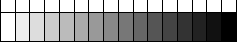
\includegraphics{Figures/ProgrammingLanguage/ReverseGrayMap}
\end{center}
%@END

%@DOC:ColorMap::ColorMap()
% Automatic documentation generated from the DynELA source code
% Do not change anything in this LaTeX file between the @DOC and the @END keywords.
\textcolor{purple}{\textbf{ColorMap::ColorMap(~)}}\label{ColorMap::ColorMap()}\index[DL]{ColorMap!ColorMap(~)}\\
Default constructor of the ColorMap class.\vspace*{-0.5em}
\begin{tcolorbox}[grow to left by=-1cm, width=\textwidth-1cm,myArgs,tabularx={l|R}]
$\hookrightarrow$ ColorMap & The new ColorMap object created by the constructor.
\end{tcolorbox}

This is the default constructor of the ColorMap class. By default, the associated color map is the deep color map.
%@END

%@DOC:ColorMap::clearColorMap()
% Automatic documentation generated from the DynELA source code
% Do not change anything in this LaTeX file between the @DOC and the @END keywords.
\textcolor{purple}{\textbf{ColorMap::clearColorMap(~)}}\label{ColorMap::clearColorMap()}\index[DL]{ColorMap!clearColorMap(~)}\\
Clears the current color map.

%@END

%@DOC:ColorMap::resetColorMap()
% Automatic documentation generated from the DynELA source code
% Do not change anything in this LaTeX file between the @DOC and the @END keywords.
\textcolor{purple}{\textbf{ColorMap::resetColorMap(~)}}\label{ColorMap::resetColorMap()}\index[DL]{ColorMap!resetColorMap(~)}\\
Reset and recomputes the color map.

%@END

%@DOC:ColorMap::setBounds(double min, double max)
% Automatic documentation generated from the DynELA source code
% Do not change anything in this LaTeX file between the @DOC and the @END keywords.
\textcolor{purple}{\textbf{ColorMap::setBounds(double min, double max)}}\label{ColorMap::setBounds(double min, double max)}\index[DL]{ColorMap!setBounds(double min, double max)}\\
Sets the boundary values of the current color map.

\begin{tcolorbox}[width=\textwidth,myArgs,tabularx={ll|R}]


\end{tcolorbox}

%@END

%@DOC:ColorMap::setLevels(int l)
% Automatic documentation generated from the DynELA source code
% Do not change anything in this LaTeX file between the @DOC and the @END keywords.
\textcolor{purple}{\textbf{ColorMap::setLevels(int l)}}\label{ColorMap::setLevels(int l)}\index[DL]{ColorMap!setLevels(int l)}\\
Sets the number of levels of the current color map.

\begin{tcolorbox}[width=\textwidth,myArgs,tabularx={ll|R}]

\end{tcolorbox}

%@END

%@DOC:ColorMap::getIntColor(double val)
% Automatic documentation generated from the DynELA source code
% Do not change anything in this LaTeX file between the @DOC and the @END keywords.
\textcolor{purple}{\textbf{ColorMap::getIntColor(double val)}}\label{ColorMap::getIntColor(double val)}\index[DL]{ColorMap!getIntColor(double val)}\\
Get the color index of a value.\vspace*{-0.5em}
\begin{tcolorbox}[grow to left by=-1cm, width=\textwidth-1cm,myArgs,tabularx={l|R}]
$\hookrightarrow$  int & The index of the color.
\end{tcolorbox}

\begin{tcolorbox}[width=\textwidth,myArgs,tabularx={ll|R}]

\end{tcolorbox}

%@END

%@DOC:ColorMap::getVec3DColor(double val, bool s)
% Automatic documentation generated from the DynELA source code
% Do not change anything in this LaTeX file between the @DOC and the @END keywords.
\textcolor{purple}{\textbf{ColorMap::getVec3DColor(double val, bool s)}}\label{ColorMap::getVec3DColor(double val, bool s)}\index[DL]{ColorMap!getVec3DColor(double val, bool s)}\\
Get the color as RGB components.\vspace*{-0.5em}
\begin{tcolorbox}[grow to left by=-1cm, width=\textwidth-1cm,myArgs,tabularx={l|R}]
$\hookrightarrow$  Vec3D & the RGB components of the color.
\end{tcolorbox}

\begin{tcolorbox}[width=\textwidth,myArgs,tabularx={ll|R}]


\end{tcolorbox}

If the color is out of range, this method returns black if the value is lower than the minimum value, white if it is larger than the highest value.
%@END

%@DOC:ColorMap::getStringColor(double val, bool s)
% Automatic documentation generated from the DynELA source code
% Do not change anything in this LaTeX file between the @DOC and the @END keywords.
\textcolor{purple}{\textbf{ColorMap::getStringColor(double val, bool s)}}\label{ColorMap::getStringColor(double val, bool s)}\index[DL]{ColorMap!getStringColor(double val, bool s)}\\
Get the color as String components.\vspace*{-0.5em}
\begin{tcolorbox}[grow to left by=-1cm, width=\textwidth-1cm,myArgs,tabularx={l|R}]
$\hookrightarrow$  String & the String components of the color.
\end{tcolorbox}

\begin{tcolorbox}[width=\textwidth,myArgs,tabularx={ll|R}]


\end{tcolorbox}

If the color is out of range, this method returns black if the value is lower than the minimum value, white if it is larger than the highest value.
%@END

%@DOC:ColorMap::getBounds(double min, double, max, int l)
% Automatic documentation generated from the DynELA source code
% Do not change anything in this LaTeX file between the @DOC and the @END keywords.
\textcolor{purple}{\textbf{ColorMap::getBounds(double min, double, max, int l)}}\label{ColorMap::getBounds(double min, double, max, int l)}\index[DL]{ColorMap!getBounds(double min, double, max, int l)}\\
Get the boundaries of the current color map.

\begin{tcolorbox}[width=\textwidth,myArgs,tabularx={ll|R}]



\end{tcolorbox}

%@END

%@DOC:ColorMap::getMax()
% Automatic documentation generated from the DynELA source code
% Do not change anything in this LaTeX file between the @DOC and the @END keywords.
\textcolor{purple}{\textbf{ColorMap::getMax(~)}}\label{ColorMap::getMax()}\index[DL]{ColorMap!getMax(~)}\\
Get the max value of the current color map.\vspace*{-0.5em}
\begin{tcolorbox}[grow to left by=-1cm, width=\textwidth-1cm,myArgs,tabularx={l|R}]
$\hookrightarrow$ double & The maximum value of the range.
\end{tcolorbox}

%@END

%@DOC:ColorMap::getMin()
% Automatic documentation generated from the DynELA source code
% Do not change anything in this LaTeX file between the @DOC and the @END keywords.
\textcolor{purple}{\textbf{ColorMap::getMin(~)}}\label{ColorMap::getMin()}\index[DL]{ColorMap!getMin(~)}\\
Get the min value of the current color map.\vspace*{-0.5em}
\begin{tcolorbox}[grow to left by=-1cm, width=\textwidth-1cm,myArgs,tabularx={l|R}]
$\hookrightarrow$ double & The minimum value of the range.
\end{tcolorbox}

%@END

%@DOC:ColorMap::getLevels()
% Automatic documentation generated from the DynELA source code
% Do not change anything in this LaTeX file between the @DOC and the @END keywords.
\textcolor{purple}{\textbf{ColorMap::getLevels(~)}}\label{ColorMap::getLevels()}\index[DL]{ColorMap!getLevels(~)}\\
Get the number of levels of the current color map.\vspace*{-0.5em}
\begin{tcolorbox}[grow to left by=-1cm, width=\textwidth-1cm,myArgs,tabularx={l|R}]
$\hookrightarrow$ int & The number of levels.
\end{tcolorbox}

%@END


